\documentclass[../../course]{subfiles}

\renewcommand\thesection{\arabic{section}}


\begin{document}

\def\freqXOne{28}
\def\freqXTwo{56}
\def\freqXThree{56.1}

\section{Generating Sequences} \label{sec:wrkGenSeqs}

First of all, we need to generate three sequences, with frequencies of:

\begin{align}
    f_{1} &= \freqXOne \si{Hz}                                  \label{eqn:freq1} \\
    f_{2} &= 2 \times \freqXOne         = \freqXTwo   \si{Hz}   \label{eqn:freq2} \\
    f_{3} &= (2 \times \freqXOne) + 0.1 = \freqXThree \si{Hz}   \label{eqn:freq3}
\end{align}

Now we need to decide whether we need to generate a \emph{sine} signal or one with
$90 \degree$ phase shift, ie, the \emph{cosine} signal. If we mix\footnote{like, real
part and imaginary part having a phase difference} \emph{sine} and \emph{cosine} we may
get a different kind of \emph{complex} sequence than if we mix \emph{sine} to \emph{sine}
or \emph{cosine} to \emph{cosine}. For our analysis, let's stick with having zero phase
shift between the signals that we are mixing. So let's just mix \emph{sine} signals with
the above frequencies.


To get the continuous feel of these sequences let's generate them with $2500$ samples.
And these signals will range from $0$ to $\frac{\pi}{4}$.


Therefore these signals will be:

\begin{align}
    x_{1}(t) =
    \begin{cases}
        \sin(2 \pi \freqXOne t) & \text{; for} \; 0 \le t \le \dfrac{\pi}{4}
    \end{cases}
    \label{eqn:seqx1}
\end{align}

\begin{align}
    x_{2}(t) =
    \begin{cases}
        \sin(2 \pi \freqXTwo t) & \text{; for} \; 0 \le t \le \dfrac{\pi}{4}
    \end{cases}
    \label{eqn:seqx2}
\end{align}

\begin{align}
    x_{3}(t) =
    \begin{cases}
        \sin(2 \pi \freqXThree t) & \text{; for} \; 0 \le t \le \dfrac{\pi}{4}
    \end{cases}
    \label{eqn:seqx3}
\end{align}

\subsection{Python Implementation} \label{lst:threeSeqs}

%python/three_sequences.py%
\begin{minted}[breaklines, autogobble, mathescape] {python}
    import numpy as np
    import pandas as pd

    X = 28
    t = np.linspace(0, np.pi / 4, 2500)

    x1 = np.sin( 2 * np.pi * X * t)
    x2 = np.sin( 2 * np.pi * (2 * X) * t)
    x3 = np.sin( 2 * np.pi * ((2 * X) + 0.1) * t)

    data = pd.DataFrame(
        {
            "x1": x1,
            "x2": x2,
            "x3": x3,
        }
    )

    data.to_csv(
        "../data/three_sequences.csv",
        sep = " ", index_label = "time"
    )
    print(data)

\end{minted}

\paragraph{Output}

\begin{minted}[breaklines, autogobble] {text}
                x1        x2        x3
    0     0.000000  0.000000  0.000000
    1     0.055264  0.110359  0.110555
    2     0.110359  0.219369  0.219754
    3     0.165116  0.325699  0.326259
    4     0.219369  0.428051  0.428765
    ...        ...       ...       ...
    2495 -0.273262 -0.525724 -0.060838
    2496 -0.219684 -0.428635  0.049885
    2497 -0.165435 -0.326311  0.159997
    2498 -0.110680 -0.220000  0.268147
    2499 -0.055586 -0.111001  0.373009

    [2500 rows x 3 columns]
\end{minted}

\subsubsection{Plots}

\begin{figure} [H]
    \centering
    \adjustbox{max width = \textwidth} {
        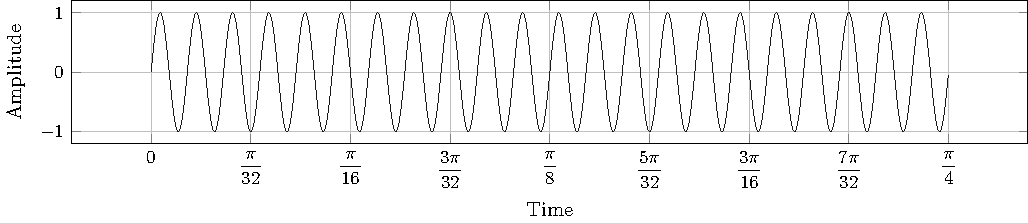
\includegraphics[height = 0.8\textheight] {tikzpics/plotSeqX1.pdf}
    }
    \captionof{figure} {Sine signal $x_{1}$ with frequency of $\freqXOne \si{Hz}$}
    \label{plt:seqx1}
\end{figure}

\begin{figure} [H]
    \centering
    \adjustbox{max width = \textwidth} {
        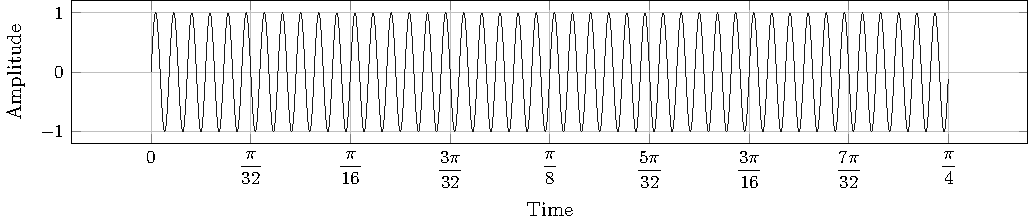
\includegraphics[height = 0.8\textheight] {tikzpics/plotSeqX2.pdf}
    }
    \captionof{figure} {Sine signal $x_{2}$ with frequency of $\freqXTwo \si{Hz}$}
    \label{plt:seqx2}
\end{figure}

\begin{figure} [H]
    \centering
    \adjustbox{max width = \textwidth} {
        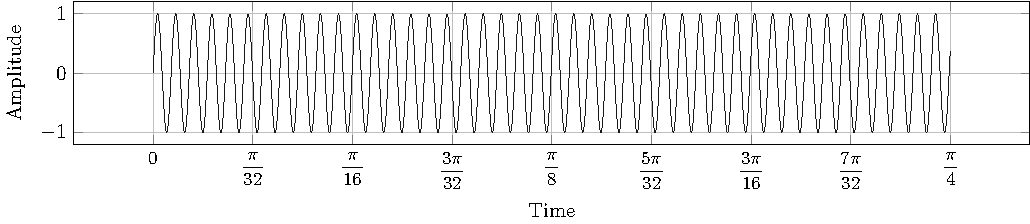
\includegraphics[height = 0.8\textheight] {tikzpics/plotSeqX3.pdf}
    }
    \captionof{figure} {Sine signal $x_{3}$ with frequency of $\freqXThree \si{Hz}$}
    \label{plt:seqx3}
\end{figure}

\end{document}
